\section{Palindromi}

U ovom odeljku pokaza\' cemo da skup svih palindromskih podstringova stringa $s$ ima zanimljivu strukturu, i da\' cemo jednostavne i efikasne algoritme koji nalaze tu strukturu.

\begin{thm}
\label{brojpalindroma}
String $s$ du\v zine $n$ ima ne vi\v se od $n$ razli\v citih nepraznih palindromskih podstringova.
\end{thm}

\textit{Dokaz.} Indukcijom po du\v zini stringa $n$. Za $n=1$ tvr\dj enje o\v cigledno va\v zi, jer string ima samo jedan palindromski podstring -- sebe samog. Neka je $n>1$. Posmatrajmo sve palindromske sufikse stringa $s$, neka najdu\v zi od njih ima du\v zinu $k$. Svaki palindromski sufiks du\v zine $l<k$ stringa $s$ se javlja i u podstringu $s_{[0,n-1)}$, zato \v sto je $s_{[n-k,n)}$ palindrom, pa je $s_{[n-l,n)} = \overline{s_{[n-k, n-k+l)}} = s_{[n-k, n-k+l)}$, \v sto je podstring jer va\v zi $0 \leq n-k \leq n-k+l \leq n-1$. Dakle, skup palindromskih podstringova za string $s$ ima najvi\v se jedan element vi\v se nego taj skup za string $s_{[0,n-1)}$, i to mo\v ze biti samo podstring $s_{[n-k,n)}$. \hfill $\square$

Jednostavan algoritam koji nalazi sve palindrome je slede\' ci. Fiksirajmo centar palindroma. Centar mo\v ze biti jedno slovo ili pozicija izme\dj u dva uzastopna slova, \v sto odgovara redom palindromima neparne i parne du\v zine. Sve dok se prvo i poslednje slovo poklapaju, pove\' cavamo granice. Oslanjamo se na ideju da, ako je $s$ palindrom du\v zine bar $2$, tada je i $s_{[1, n-1)}$ tako\dj e palindrom. Algoritam zato vra\' ca samo maksimalne palindrome, tj. palindrome koji se ne mogu pro\v siriti i sa leve i sa desne strane istovremeno.

\noindent
\begin{minipage}[l]{\textwidth}
\lstinputlisting[language=C++, title={\textit{Algoritam za nala\v zenje svih maksimalnih palindromskih podstringova}}, style=customcpp]{cpp/palin-simple.cpp}
\end{minipage}

Glavni nedostatak algoritma je njegova vremenska slo\v zenost, koja u najgorem slu\v caju iznosi $\Theta(n^2)$, i posti\v ze se za string $s = a^n$.

\subsection{Manacher-ov algoritam}

Pre nego \v sto opi\v semo sam algoritam, da bismo ga pojednostavili svedimo problem nala\v zenja maksimalnih palindroma na problem nala\v zenja maksimalnih palindroma neparne du\v zine. Ovo radimo tako \v sto od stringa $s$ du\v zine $n$ pravimo string $p$ du\v zine $2n+1$, $p = \$s_0\$s_1\$\ldots \$s_{n-1}\$$, gde je $\$$ karakter koji se ne javlja u stringu $s$. String $p$ ne sadr\v zi parne palindrome, jer se srednja dva karaktera sigurno ne poklapaju -- jedan od njih \' ce uvek biti $\$$, a drugi ne\' ce. Sa druge strane, palindrom sa centrom u karakteru $\$$, osim na krajevima, odgovara palindromu parne du\v zine u stringu $s$, dok palindrom sa centrom u karakteru razli\v citom od $\$$ odgovara palindromu neparne du\v zine u stringu $s$. Konkretno, palindrom $p_{[l,r)}$ odgovara palindromu $s_{[\frac{l}{2}, \frac{r-1}{2})}$. Uzimamo u razmatranje samo neparne palindrome u $p$ koji po\v cinju i zavr\v savaju se sa $\$$ i imaju du\v zinu bar $3$.

Manacher-ov algoritam koristi ideju vrlo sli\v cnu Z-algoritmu. Za svaku poziciju stringa $p$ du\v zine $m$ algoritam nalazi radijus $q_i$, koji zna\v ci da maksimalni palindrom sa centrom u $i$ ima du\v zinu $2q_i+1$. Algoritam redom ra\v cuna vrednosti $q_i$ i odr\v zava prozor sa najve\' cim desnim krajem koji odgovara nekom maksimalnom palindromu. Ovaj prozor se onda mo\v ze iskoristiti da se na\dj e donja granica za vrednost $q_i$. Ukoliko je $s_{[l,r]}$ palindrom (obratiti pa\v znju da sada obuhvatamo i desni kraj intervala), onda za $i > \frac{r+l}{2}$ va\v zi $q_i \geq q_i' = \min(q_{r+l-i}, r-i)$ -- po\v sto je $s_{[l,r]}$ palindrom, onda je podstring $s_{[i-q_i', i+q_i']}$ ceo sadr\v zan u $s_{[l,r]}$ i jednak podstringu $\overline{s_{[r+l-i-q_i', r+l-i+q_i']}}$, koji je palindrom, odakle sledi da je $q_i \geq q_i'$.

\noindent
\begin{minipage}[l]{\textwidth}
\lstinputlisting[language=C++, title={\textit{Manacher-ov algoritam}}, style=customcpp]{cpp/manacher.cpp}
\end{minipage}

\noindent \textbf{Primer.} Ilustracije radi, zanemarimo uba\v cene karaktere $\$$, odnosno, radimo samo sa neparnim palindromima. Posmatrajmo string \texttt{xabcbazyzabcbazyap} i neka je $i=11$, kao na slici. Do ovog trenutka palindromski prozor sa najve\' cim desnim krajem je prozor $[l,r] = [1,13]$. Ovaj palindromski prozor reflektuje sve svoje podstringove, pa se podstring sa centrom u $r-l+i$ reflektuje u podstring sa centrom u $i$.

\begin{figure}[H]
    \centering
    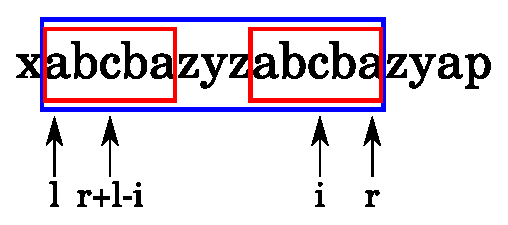
\includegraphics[width=50mm]{../img/manacher1.eps}
    \caption*{\textit{Ilustracija Manacher-ovog algoritma}}
\end{figure}

Svaki palindrom koji je u celosti sadr\v zan u nekom palindromskom prozoru \' ce se ponovo reflektovati u palindrom, \v sto nam ovde omogu\' cava da za palindromski centar $i$ postavimo donju granicu vrednosti $z_i' = 2$. Nakon postavljanja ove po\v cetne vrednosti poku\v savamo da pro\v sirimo palindrom. Ispostavlja se da se palindrom sa ovim centrom mo\v ze pro\v siriti za jo\v s dva slova, odnosno, va\v zi\' ce $z_i = 4$.

Dokaz da ovaj algoritam ima vremensku slo\v zenost $O(n)$ je sli\v can dokazu kod Z-algoritma. Doka\v zimo da se vrednost $r$ pove\' ca za bar jedan u svakoj iteraciji \textit{while} petlje. U slu\v caju da je $i + q_i' < r$, \textit{while} petlja \' ce izvr\v siti ta\v cno $0$ iteracija po\v sto je $q_i = q_i'$. U suprotnom bismo dobili, na osnovu refleksije unutar palindroma $s_{[l,r]}$ da se palindrom sa centrom u $r+l-i$ tako\dj e mo\v ze pro\v siriti za bar jedno slovo, \v sto je nemogu\' ce jer je njegova vrednost ta\v cno izra\v cunata. Drugi slu\v caj je kad je $i + q_i' \geq r$, tada \' ce, u slu\v caju da se palindrom sa centrom u $i$ pro\v siri sa $k$ iteracija \textit{while} petlje, za isto toliko pove\' cati vrednost $r$. 

\subsection{Palindromsko stablo}

Palindromsko stablo, poznato i pod imenom \textit{eertree}, je struktura podataka koja za dati string $s$ nalazi sve palindrome u stringu i omogu\' cuje njihovo efikasno pretra\v zivanje i obradu. Svaki \v cvor palindromskog stabla je jedan jedinstven neprazan palindrom. Pored ovih, postoje dva specijalna \v cvora koji odgovaraju palindromu du\v zine $0$, tj. stringu $\epsilon$, kao i fiktivnom palindromu $\eta$ du\v zine $-1$. Ovaj palindrom zadovoljava slede\' cu osobinu: ako je $x \in \Sigma$, onda je $x\eta x = x$. Svaki \v cvor ima izlazne grane sa labelama iz $\Sigma$. Ako grana polazi iz \v cvora $p$ i ima labelu $x$, onda ta grana ide ka \v cvoru $xpx$. Pored ovih grana, \v cvorovi imaju i sufiks grane -- sufiks grana iz \v cvora $p$ ide ka najdu\v zem palindromu koji je pravi sufiks palindroma $p$, ukoliko takav ne postoji, sufiks grana ide ka $\epsilon$. Kod ovog \v cvora sufiks grana ide ka \v cvoru $\eta$, dok se za \v cvor $\eta$ sufiks grana ne defini\v se. O\v cigledno, sufiks grane formiraju strukturu obrnutog korenskog stabla sa korenom u $\eta$, dok izlazne grane formiraju dva korenska stabla, jedno sa korenom u $\eta$, a drugo sa korenom u $\epsilon$, jer svi ostali \v cvorovi imaju jedinstvenu ulaznu granu, i to je grana sa labelom koja odgovara njihovom prvom tj. poslednjem slovu.

\subsubsection{Algoritam za konstrukciju}

Na osnovu teoreme \ref{brojpalindroma} imamo da je broj \v cvorova palindromskog stabla ne vi\v se od $n+2$, pa je memorijska slo\v zenost cele strukture $O(n)$. Pored navedenih grana, svaki \v cvor \' ce eksplicitno pamtiti i du\v zinu palindroma koji predstavlja.

\noindent
\begin{minipage}[l]{\textwidth}
\lstinputlisting[language=C++, title={\textit{Struktura \v cvora palindromskog stabla}}, style=customcpp]{cpp/eertree_node.h}
\end{minipage}

Glavni algoritam \' ce, pored tra\v zenog stabla, na\' ci i \v cvor koji odgovara najdu\v zem sufiksu koji je palindrom za svaki prefiks stringa $s$, odnosno, \v cvor $p_i$ odgovara najdu\v zem sufiksu koji je palindrom stringa $s_{[0,i)}$. Sve ove vrednosti, kao i samo palindromsko stablo ra\v cunamo redom za sve prefikse stringa $s$. Iz dokaza teoreme \ref{brojpalindroma} znamo da je ovaj skup palindroma jednak skupu svih palindroma koji se javljaju u $s$. Inicijalizujemo algoritam kreiranjem dva \v cvora $\epsilon, \eta$ i postavljanjem $p_0 = \epsilon$. Zatim, svaki put kad dodajemo novo slovo stringa $s$, prvo ispitujemo da li se prethodno najdu\v zi sufiks palindrom mo\v ze pro\v siriti novim slovom $c$. Ukoliko mo\v ze, onda je novi palindrom upravo taj pro\v siren slovom $c$, ina\v ce, ispitujemo dalje kre\' cu\' ci se po sufiks vezama. Kada na\dj emo prvi sufiks $t$ koji se mo\v ze pro\v siriti sa obe strane karakterom $c$, zaustavljamo se. Ukoliko \v cvor $ctc$ ve\' c postoji, ne radimo ni\v sta, ina\v ce mu moramo izra\v cunati sufiks vezu. Ukoliko je $t = \eta$, novi palindrom ima samo jedno slovo, odnosno $c$ se javlja prvi put u stringu i njegova sufiks veza ide ka \v cvoru $\epsilon$, ina\v ce, kre\' cemo od sufiks veze \v cvora $t$ i tra\v zimo najdu\v zi sufiks koji se mo\v ze pro\v siriti slovom $c$. Takav \' ce sigurno postojati jer se slovo $c$ ne javlja prvi put u stringu, pa \' ce bar $\eta$ mo\' ci da se produ\v zi. Ako je $q$ takav palindrom, onda je sufiks veza za novi \v cvor upravo $cqc$.

\noindent
\begin{minipage}[l]{\textwidth}
\lstinputlisting[language=C++, title={\textit{Algoritam za konstrukciju palindromskog stabla}}, style=customcpp]{cpp/eertree.cpp}
\end{minipage}

\noindent \textbf{Primer.} Neka je string $s$ za koji pravimo palindromsko stablo jednak \texttt{aabaa}. Posmatrajmo \v sta se de\v sava u trenutku kada je $i=4$, odnosno, dodajemo poslednje slovo stringa. Do tog trenutka bi\' ce prona\dj ena $4$ neprazna palindromska podstringa, to su $a,b,aa,aba$. Sufiks veze za $a$ i $b$ idu ka \v cvoru $\epsilon$, dok sufiks veze za $aa$ i $aba$ idu ka \v cvoru $a$. Podsetimo se da izlazne grane uvek idu od \v cvora $t$ ka \v cvoru $xtx$ za neki palindrom $t$ i slovo $x$.

\begin{figure}[H]
    \centering
    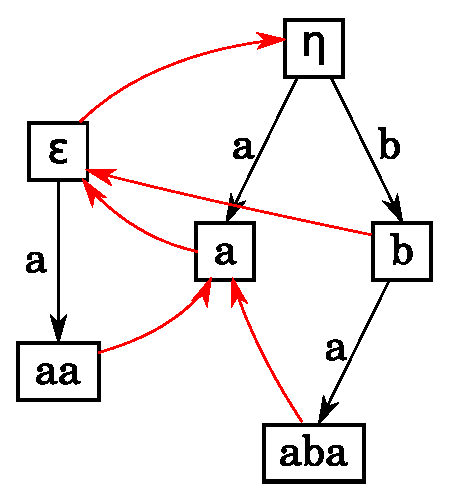
\includegraphics[width=50mm]{../img/eertree1.eps}
    \caption*{\textit{Palindromsko stablo za string aaba}}
\end{figure}

Sada dodajemo slovo $a$ na kraj stringa. Prethodni najdu\v zi sufiks palindrom je bio $aba$, i njegovo pojavljivanje se mo\v ze produ\v ziti sa obe strane slovom $a$, pa je za $i+1=5$ najdu\v zi sufiks palindrom $aabaa$. Izlazna grana sa labelom $a$ iz \v cvora $aba$ ne postoji, pa dodajemo novi \v cvor. Sada je potrebno odrediti sufiks vezu za ovaj \v cvor. Kre\' cemo od sufiks veze \v cvora $aba$, \v sto je \v cvor $a$ i tra\v zimo palindrom \v cije se pojavljivanje kao sufiks stringa $s_{[0,i)}$ mo\v ze pro\v siriti sa obe strane slovom $a$. Prvi takav \v cvor je \v cvor $\epsilon$, pa sufiks veza ide ka \v cvoru $a\epsilon a$ odnosno $aa$.

\begin{figure}[H]
    \centering
    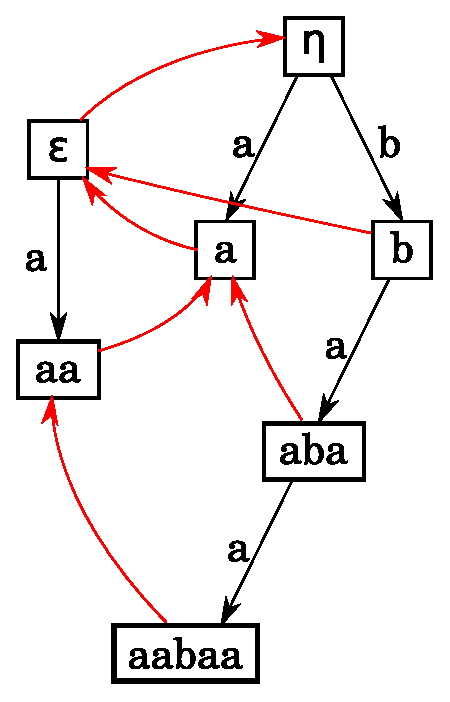
\includegraphics[width=50mm]{../img/eertree2.eps}
    \caption*{\textit{Palindromsko stablo za string aabaa}}
\end{figure}

Vremenska slo\v zenost algoritma je $O(n)$. To se mo\v ze dokazati ako posmatramo vrednost $5i-len(t)- len(link(t))$. U svakoj iteraciji neke od \textit{while} ili \textit{for} petlji se ova vrednost pove\' cava. Za \textit{while} petlje je to o\v cigledno. Za \textit{for} petlju primetimo da, ukoliko je najdu\v zi sufiks palindrom nekog stringa imao du\v zinu $l$, ako se doda jedno slovo na kraj stringa, ta du\v zina mo\v ze postati najvi\v se $l+2$, i isto va\v zi za du\v zinu drugog najdu\v zeg sufiks palindroma (tj. sufiks veze), pa se $len(t)- len(link(t))$ pove\' cava za najvi\v se $4$, a $5i$ se pove\'cava za ta\v cno $5$. Kako je po\v cetna vrednost izraza $1$, a na kraju ne prelazi $5n$, ukupan broj izvr\v senja svih petlji je $5n$, pa algoritam ima vremensku slo\v zenost $O(n)$. 

\subsubsection{Primene}

\noindent
\textbf{Najdu\v zi palindromski podstring}

Palindromsko stablo re\v sava ovaj problem u istoj vremenskoj slo\v zenosti kao Manacher-ov algoritam, odnosno u $O(n)$. Dovoljno je za sve \v cvorove stabla uzeti vrednost $len(u)$ i vratiti onaj koji ima najve\' cu. Pozicija palindroma u stringu se mo\v ze na\' ci ispitivanjem za koje $i$ je $p_i = u$. U tom slu\v caju se palindrom nalazi na poziciji $s_{[i-len(u), i)}$.

\noindent
\textbf{Ukupan broj palindroma}

Na\dj imo za svaki \v cvor stabla $t$ sufiks veza dubinu $d(t)$, odnosno broj \v cvorova na putu od tog \v cvora do nekog \v cvora sa $len = 1$. Ovo \' ce nam za palindrom $t$ dati broj sufiksa stringa $t$ koji su palindromi. Re\v senje za ceo string $s$ je $\sum_{i=1}^n d(p_i)$.

Prethodni problemi se mogu efikasno re\v siti i Manacher-ovim algoritmom. Me\dj utim, on nije dovoljan za naredne.

\noindent
\textbf{Broj razli\v citih palindroma}

Po definiciji palindromskog stabla, broj razli\v citih palindroma pozitivne du\v zine je broj \v cvorova stabla umanjen za $2$, jer ne ra\v cunamo \v cvorove $\epsilon$ i $\eta$.

\noindent
\textbf{Ispitivanje pojavljivanja palindroma}

Ukoliko ispitujemo da li se string parne du\v zine oblika $\overline{u}u$ javlja u $s$, mo\v zemo samo pratiti izlazne grane sa labelama koje odgovaraju slovima stringa $u$, po\v cev od \v cvora $\epsilon$. Za neparne palindrome oblika $\overline{u}xu$, kre\' cemo iz $\eta$ i kre\' cemo se labelama $xu$.